	\noindent \textbf{RQ2:}\textbf{ Can code, log and developer related metrics help in explaining the stability of logs?}
	\\\\
\noindent \textbf{Motivation}

In RQ1, we find that 45\% of logs are changed at-least once in three of out studied systems. This affects the log processing tools which run on these studied systems, making developers spend more time on maintenance of those tools. Hence, there is a need to identify these non-stable logs to simplify the job of developers. It can also benefit log processing tool developers to develop more robust applications making them more stable.

To identify these non-stable logs we use code, log and developer metrics. We use these metrics because this data can be extracted from control version systems (CVS) easily by developers. It also benefits log processing tool developers as do not need domain knowledge about the system to understand these metrics.\\
%
%can be extracted from control versions systems by developersthem.  \\


\noindent \textbf{Approach}
\begin{table*}
\centering
	\caption{Taxonomy of metrics considered for model construction}
	
	\label{tba:Taxonomy}
		\begin{tabular}{|c|c|c|>{\raggedright}p{1\columnwidth}|}
			\hline 
			Dimension & Metrics & Values & Definition (d) -- Rationale (r)\tabularnewline
			\hline 
			\hline 
			\multirow{12}{*}{Code Metrics} & \multirow{2}{*}{Log revision count} & \multirow{2}{*}{Numeric } & d: The number of prior commits which had log changes. \tabularnewline
			\cline{4-4} 
			&  &  & r: This helps to identify if the file is prone to log changes.\tabularnewline
			\cline{2-4} 
			& \multirow{2}{*}{New file} & \multirow{2}{*}{Boolean (0 -1)} & d: Check if the log is added in a new file (i.e., newly committed )\tabularnewline
			\cline{4-4} 
			&  &  & r: This helps to identify which logs where added later in subsequent commits.\tabularnewline
			\cline{2-4} 
			& \multirow{2}{*}{Total revision count} & \multirow{2}{*}{Numeric} & d: Total number of commits made to the file before the log is
			added. This value is 0 for logs added in the initial commit but not for logs added overtime. \tabularnewline
			\cline{4-4} 
			&  &  & r: This helps to find out if the file is changed heavily which can
			result in log changes~\cite{Characterizinglogs}. \tabularnewline
			\cline{2-4} 
			& \multirow{2}{*}{Code churn in commit} & \multirow{2}{*}{Numeric} & d: The code churn of the commit in which a log is added. \tabularnewline
			\cline{4-4} 
			&  &  & r: Log changes are correlated to code churn in files~\cite{EMSEIAN}. \tabularnewline
			\cline{2-4} 
			& \multirow{2}{*}{Variables declared} & \multirow{2}{*}{Numeric} & d: The number of variables which are declared before the log statement.
			(we limit to 20 lines before log statement).\tabularnewline
			\cline{4-4} 
			&  &  & r: When new variables are declared, developers may log the new variables to obtain more information~\cite{Characterizinglogs}. \tabularnewline
			\cline{2-4} 
		 			
			& \multirow{2}{*}{SLOC} & \multirow{2}{*}{Numeric} & d: The number of lines of code in the file.\tabularnewline
			\cline{4-4} 
			&  &  & r: Large files have more functionality and are more prone to changes~\cite{zhang2009investigation} and more log changes~\cite{Characterizinglogs,EMSEIAN}. \tabularnewline
			\hline 
			\multirow{10}{*}{Log metrics} & \multirow{2}{*}{Log context} & \multirow{2}{*}{Categorical} & d: Identify the block in which a log is added. (i.e., `if',
			`if-=else', `try-catch', `exception', `throw', `new function').\tabularnewline
			\cline{4-4} 
			&  &  & r: Prior research finds that logs are mostly used in assertion checks, logical branching, return value checking, assertion checking~\cite{Fu1}. \tabularnewline
			\cline{2-4} 
			& \multirow{2}{*}{Log level} & \multirow{2}{*}{Categorical} & d: Identify the log level (verbosity) of the added log (i.e., `info',
			`error', `warn', `debug', `trace' and `trace').\tabularnewline
			\cline{4-4} 
			&  &  & r: Developers spend significant amount of time in adjusting the verbosity
			of logs~\cite{Characterizinglogs}. \tabularnewline
			\cline{2-4} 
			& \multirow{2}{*}{Log variable count} & \multirow{2}{*}{Numerical} & d: Number of variables logged.\tabularnewline
			\cline{4-4} 
			&  &  & r: Over 62\% of logs add new variables~\cite{Characterizinglogs}. Hence fewer variables in the initial log statement might result
			in addition later. \tabularnewline
			\cline{2-4} 
			& \multirow{2}{*}{Log text length} & \multirow{2}{*}{Numerical} & d: Number of text phrases logged (i.e., we count all text present
			between a pair of quotes as one phrase).\tabularnewline
			\cline{4-4} 
			&  &  & r: Over 45\% of logs have modifications to static context~\cite{Characterizinglogs}. Logs with fewer phrases might be subject to changes later to provide better explanation.\tabularnewline
			\cline{2-4} 
			& \multirow{2}{*}{Log density} & \multirow{2}{*}{Numerical} & d: Ratio of number of log lines to the source code lines in the file.\tabularnewline
			\cline{4-4} 
			&  &  & r: Research has found that there is on average one log line per 30 lines of code~\cite{Characterizinglogs}. If it is less it suggests there may be additions in later commits.\tabularnewline
			\hline 
		\multirow{12}{*}{Developer Metrics} & \multirow{2}{*}{Resolution time} & \multirow{2}{*}{Numerical} & d: The time it takes for the issue to get fixed. It is defined as
		the time it takes since an issue is opened until closed. \tabularnewline
		\cline{4-4} 
		&  &  & r: More resolution time might suggest a more complex fix with more log churn. \tabularnewline
		\cline{2-4} 
		& \multirow{2}{*}{Number of developers involved} & \multirow{2}{*}{Numeric} & d: Total number of unique developers who comment on the issue report
		on JIRA.\tabularnewline
		\cline{4-4} 
		&  &  & r: Components with many unique authors likely lack strong ownership,
		which in turn may lead to more defects~\cite{mcintosh2014impact} and change logs~\cite{EMSEIAN}. \tabularnewline
		\cline{2-4} 
& \multirow{2}{*}{Number of comments} & \multirow{2}{*}{Numeric} & d: Total number of discussion posts on the issue. \tabularnewline
\cline{4-4} 
&  &  & r: Number of comments is correlated to the resolution time of issue
reports~\cite{giger2010predicting}. More comments	may also indicate the issue is more complex resulting in more code churn and log changes. \tabularnewline
\cline{2-4}
		& \multirow{2}{*}{Developer experience} & \multirow{2}{*}{Numeric} & d: The number of commits the developer has made prior to this commit. \tabularnewline
		\cline{4-4} 
		&  &  & r: Research has shown that experienced developers might take up more
		complex issues~\cite{rahman2011ownership} and therefore may leverage logs more~\cite{EMSEIAN}. \tabularnewline
		\cline{2-4} 
		& \multirow{2}{*}{Issue type} & \multirow{2}{*}{Categorical} & d: Identify the type of issue, i.e., `Bug', `Improvement', `Task',
		`New Feature', `Sub-Task', `Test'. \tabularnewline
		\cline{4-4} 
		&  &  & r: Some issue types might have higher code churn than others (example:
		Bug and New features might have more code churn when compared to Sub-Tasks) and are committed faster.\tabularnewline
		\cline{2-4} 
		& \multirow{2}{*}{Priority type} & \multirow{2}{*}{Categorical} & d: Identify the priority of the issue i.e., `Critical', `Blocker',
		`Major', `Minor' and `Trivial'\tabularnewline
		\cline{4-4} 
		&  &  & r: Research has shown that priority of issue affects resolution time
		of bug fixes~\cite{MarkFixTime}. A Higher priority indicates the issue will be fixed faster
		with log changes. \tabularnewline
		\hline 
	\end{tabular}\protect

\end{table*}



To find the stability of logs in our studied systems, we extract code and log churn metrics from the Git repository and developer metrics from JIRA. We use code churn metrics because prior work has linked logs to development knowledge and issue reports~\cite{IanIcesm}.

Table~\ref{tba:Taxonomy} lists all the metrics we collect for each dimension. We define each metric and the rationale behind the choice of each metric.  We collect the code and log churn metrics when a log is added into the studied system and track the log. If it is changed in subsequent revisions we flag the log as changed and record it. 


%To build prediction models it is necessary to track the changes to logs within the time frame of our study. To achieve this we built a tool which tracks the changes made to each log.  
%
%Since no prior work exists( to our best knowledge ) to predict the stability of logs, we use the code and developer related metrics  to explain the stability of logs. Table ( make table for metrics) explain the different metrics in each category and the rationale for using them. Figure ( make figure explaining process of when log metrics collected and log tracked) shows the process of when metrics are collected and tracking of log. 

%	
%\textbf{Random Forest:} We build random forest to help in predicting the log changes in the revisions of studied systems. A random forest is collection of largely uncorrelated decision trees where they trees combine their results to form a generalized predictor (ref paper). Random forests use bagging strategy (breiman 1996), where the decision trees are constructed using a bootstrap sample dataset. The trees are independent i.e, they do not reply on the earlier trees. In addition to this, random forests split each node using the best among a subset of predictors randomly chosen at that node (breiman 2001). This makes the random forests robust against over-fitting and are more accurate than other tree algorithms (Brieman 2001). 

\subsubsection*{\textbf{Model construction}}

We build random forest models to explain the stability of logs in our studied systems. A random forest is a collection of largely uncorrelated decision trees in which the results of all trees are combined to form a generalized predictor~\cite{Albert2008424}. In our model the code, log and developer metrics are the explanatory variables and the dependent class variable is if the log is changed or not (i.e., 'False' for not changed and 'True' for changed).

Figure~\ref{fig:ModelCreationLogGeanology} provides an overview of the four construction steps (C1 to C4) for building a random forest model and evaluating the model. We adopt the statistical tool R to model our data and use the `RandomForest' package to generate the random forests.\\

\textbf{\textsl{(C1 - Correlation analysis) }}

Correlation analysis is necessary to remove the highly correlated metrics from our dataset. Collinearity between metrics can affect the performance of a model because, small changes in one metric can affect the values of other metrics causing large changes on the dependent class variable.

 We use Spearman rank correlation~\cite{spearmanbook} to remove these correlated metrics from our data. Spearman rank correlation assesses how well two metrics can be described by a monotonic function. We use Spearman rank correlation instead of Pearson~\cite{pearsonbook} because Spearman is resilient to data that is not normally distributed. We use the function `varclus' in R to perform the correlation analysis.

Figure~\ref{fig:SpearmanActiveMQ} shows the hierarchically clustered Spearman $\rho $ values in ActiveMQ project. The solid horizontal lines indicate the correlation value of the two metrics that are connected by the vertical branches that descend from it.  We exclude one metric from the sub-hierarchies which have correlation $|\rho| > 0.7 $. The gray line indicates our cutoff value ($ | \rho | $ = 0.7). We use cutoff value of ($ | \rho | $ = 0.7) as used by prior research~\cite{ShaneOLS} to remove the correlated metrics before building our model. \\

\begin{figure}
	\centering
	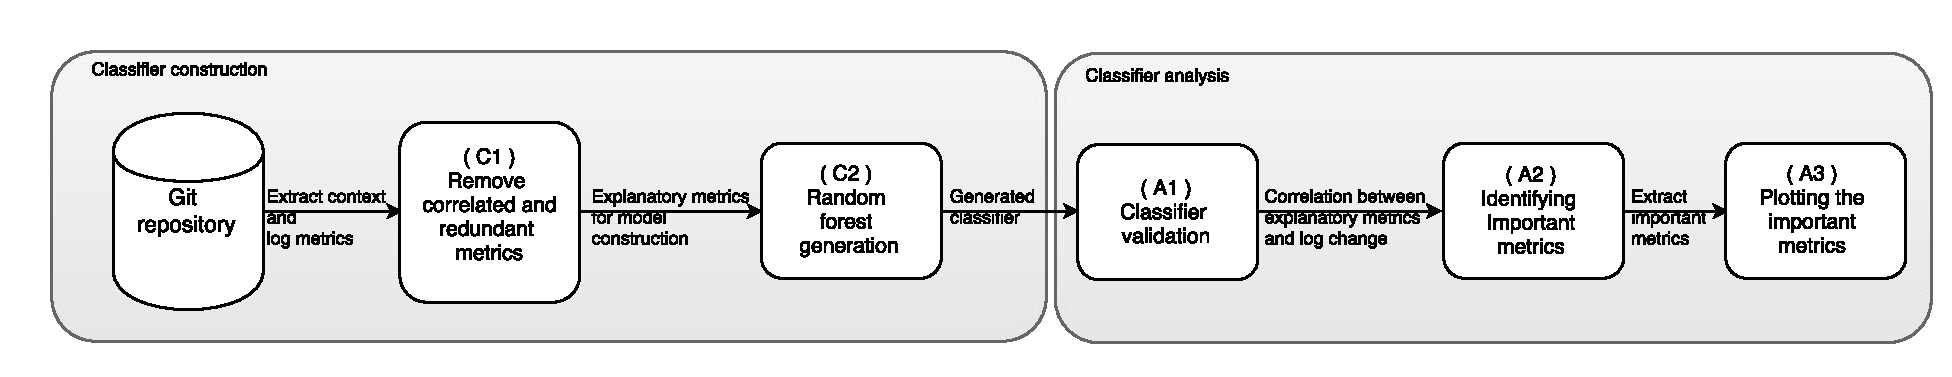
\includegraphics[width=1\columnwidth]{ModelCreationLogGeanology}
	\caption{Overview of Model construction(C) and Evaluation}
	\label{fig:ModelCreationLogGeanology}
\end{figure}  




\begin{figure}
	\centering
	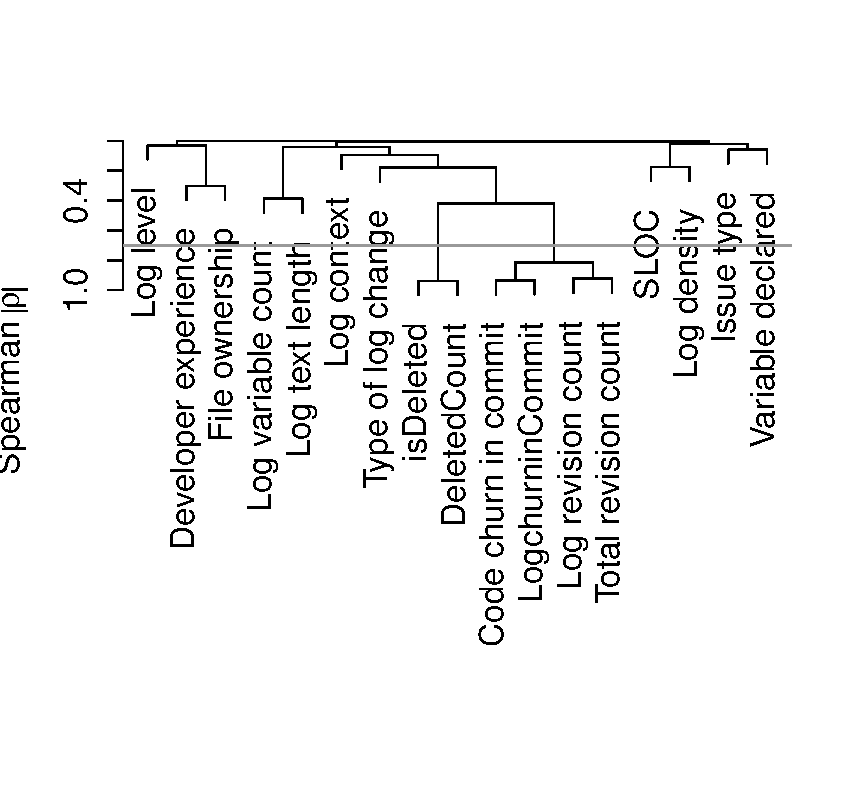
\includegraphics[height=1\columnwidth,width=0.9\columnwidth]{SpearmanActiveMQ}
 \vspace*{-1cm}	\caption{Hierarchical clustering of variables according to Spearman’s $\rho$ in ActiveMQ}
	\label{fig:SpearmanActiveMQ}
\end{figure}


\textbf{\noindent\textsl{(C2 - Random forest generation)}}

After we eliminate the correlated metrics from our datasets, we construct the random forest model.`Random forest' is a black-box ensemble classifier, which operates by constructing a multitude of decision trees on the training set and uses this to classify the testing set.
\begin{figure}
	\centering
	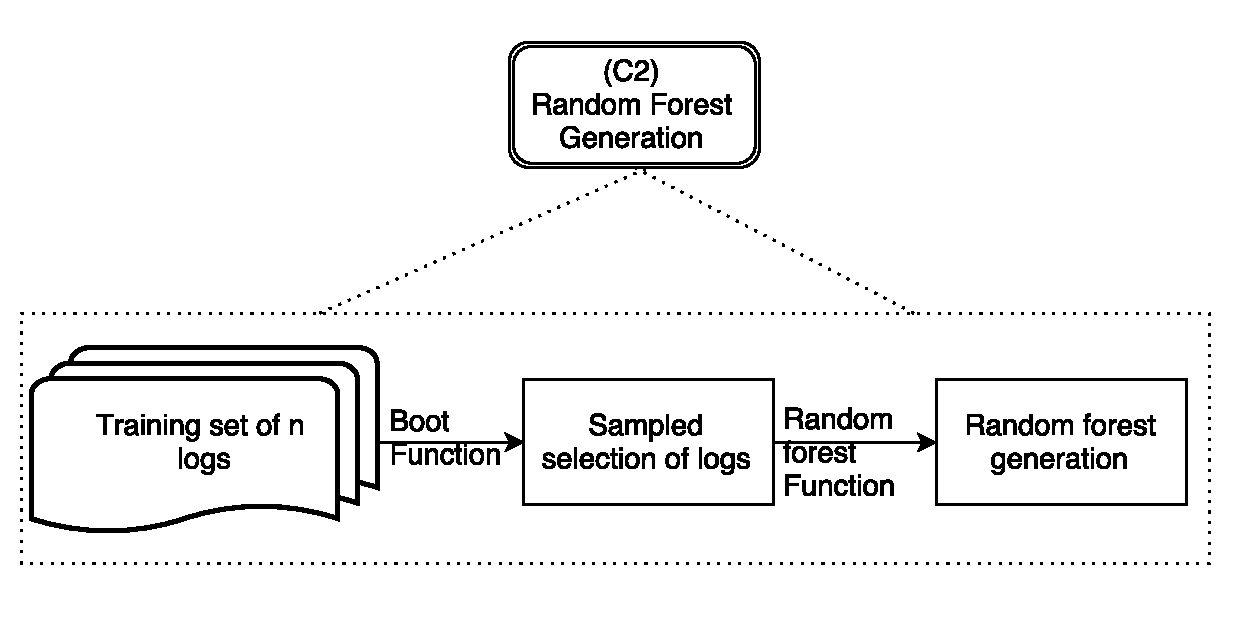
\includegraphics[height=.7\columnwidth,width=1\columnwidth]{BootRandomForest}
	\caption{ Overview of random forest generation in C2}
	\label{fig:BootRF}
\end{figure}


Given a dataset of \textsl{n} logs for training, $ D = \{ (X_{1}Y_{1},...,(X_{n}Y_{n}) \} $ where $X_{i}, i = 1...n$, is a vector of descriptors (i.e, explanatory metrics) and $Y_{i}$ is the flag which indicates whether a log is changed or not, the algorithm follows these steps and is shown in Figure~\ref{fig:BootRF}.
\begin{enumerate}
\item From the training set of \textsl{n} logs, a random sample of \emph{n} components is selected with replacement (i.e., bootstrap sample)~\cite{ShaneOLS}.

We use the `boot' function from the `boot' package in R to generate bootstrap samples. The boot function generates a set of random indices, with replacement from the integers 1:\emph{n}.

\item From the sampled selection, a tree is grown with one difference compared to normal decision trees. The random forest is split at each node using the best among subset of predictors, rather than all. This strategy helps to make the random forests more robust against over-fitting~\cite{breiman1996bagging}.

 We use the `randomForest' function from the `randomForest' package in R to generate the random forest model. 


\item The above steps are repeated until \textsl{M} such models are grown.
\item Predict new data by aggregating the prediction of the $M$ models generated.
\end{enumerate}  

\begin{table}[t]
\centering
	\begin{tabular}{|>{\raggedright}p{0.1\columnwidth}>{\raggedright}p{0.2\columnwidth}|l>{\raggedright}p{0.2\columnwidth}|}
		\hline 
		\multicolumn{1}{|>{\raggedright}p{0.03\columnwidth}}{\multirow{2}{0.03\columnwidth}{}} &  & \multicolumn{2}{c|}{Predicted}\tabularnewline
		&  & Log has changed & Log has not-changed\tabularnewline
		\hline 
		\multirow{2}{0.03\columnwidth}{Actual} & Log has changed  & TP (True Positive)  & FN (False Negative ) \tabularnewline
		& Log has not-Changed  & FP (False Positive )  & TN (True Negative) \tabularnewline
		\hline 
	\end{tabular}\protect\caption{Confusion Matrix}
	
	
	\label{tba:ConfusionMatrix} 
\end{table}

%\begin{table}[tb]
%	
%	
%	\begin{tabular}{>{\raggedright}p{0.45\columnwidth}|ll}
%		\cline{1-3}     & \multicolumn{1}{c}{Predicted log is changed}  &  \multicolumn{1}{c}{Predicted log is not-changed}	   \\ \cline{1-3}   
%		
%		Actual log is changed      & TP (True Positive)       &  FN (False Negative )     \\
%		
%		Actual log is not-Changed    & FP (False Positive )      &    TN (True Negative)   \\ \cline{1-3}
%	\end{tabular}
%	\caption{Confusion Matrix}
%	\label{tba:ConfusionMatrix}
%\end{table}

\textbf{
\noindent \textsl{(C3 - Model evaluation)}}

After we build the random forest model, we evaluate the performance of our model using precision, recall, F-measure and Brier Score. All these measures are functions of the confusion matrix as shown in Table~\ref{tba:ConfusionMatrix} and are explained below.

\textsl{Precision (P)} measure the correctness of our model in predicting which log will undergo a change in the future. It is defined as the number of logs which were accurately predicted as changed over all logs predicted to have changed as explained in Equation~\ref{f:precision}.   \\
	 \begin{equation}
 P =  \dfrac{TP}{TP + FP } 
 \label{f:precision}
	 \end{equation}	
	 
\textsl{Recall (R)} measure the completeness of our model. A model is said to be complete if the model can predict all the logs which will get changed in our dataset. It is defined as the number of logs which were accurately predicted as changed over all logs which actually change as explained in Equation~\ref{f:recall}.
	 \begin{equation}
	 R =  \dfrac{TP}{TP + FN } 
	 \label{f:recall}
	 \end{equation}	
	 
\textsl{F-Measure} is the harmonic mean of precision and recall, combining the inversely related measure into a single descriptive statistic as shown in Equation~\ref{f:Fmeasure}~\cite{F-Measure}.
	 \begin{equation}
	 F =  \dfrac{2 \times P \times R}{P + R } 
	 \label{f:Fmeasure}
	 \end{equation}	
	 
\textsl{Brier Score (BS)} is a measure of the accuracy of the predictions in our model. It is the mean squared error of the probability forecasts~\cite{wilks2011statistical}. The most common formulation of Brier Score is shown in Equation~\ref{f:BS}, where $f_{t}$ is the probability that was predicted, $o_{t}$ is the actual outcome of the event at the instance $t$ (0 if log is not changed and 1 if it is changed), and $N$ is the number of forecasting instances. 

If the predicted value is 70\% and the log is changed, the Brier Score is 0.09 (lower the Brier score, the more likely the event will occur). It reaches 0.25 for random guessing (i.e., predicted value is 50\%) and it is 0 when predicted value is 100\% and the log is not changed. 

	 \begin{equation}
	 BS =  \dfrac{1}{N}\Sigma_{t=1}^{N} (f_{t} - o_{t} )^{2} 
	 \label{f:BS}
	 \end{equation}	

The model performance measure, described previously only provide insight into how the random forest models fit the observed dataset, but it may overestimate the performance of the model if it is over-fit. We take performance overestimation (i.e., \textsl{optimism} ) into account by by subtracting the bootstrap averaged optimism~\cite{ShaneOLS} from the initial performance measure. The \textsl{optimism} of the performance measures are calculated as follows:
\begin{enumerate}
	\item From the original dataset with \textsl{n} records, select a bootstrap sample with \textsl{n} components with replacement.
	\item Build random forest using the bootstrap sample.
	\item Apply the model built from bootstrap data on both the bootstrap and original data sample, calculating precision, recall, F-measure and Brier score for both data samples.
	\item Calculate \textsl{Optimism} by subtracting the performance measures of the bootstrap sample against the original sample. 	
\end{enumerate}

	The above process is repeated 1,000 times and the average (mean) \textsl{optimism} is calculated. Finally, we calculate \textsl{optimism-reduced} performance measures for precision, recall, F-measure and Brier score by subtracting the averaged optimism of each measure, from their corresponding original measure.  The smaller the optimism values, the more stable that the original model fit is.
	\\

\textbf{\noindent \textsl{(C4 - Importance of each metric in relation to log stability)}}
To find the importance of each metric in a random forest model, we use a permutation test. In this test, the model built using the bootstrap data (i.e., two thirds of the original data) is applied to the test data(i.e., remaining one third of the original data).  

Then, the values of the $X_{i}$th metric of which we want to find importance for, are randomly permuted in the test dataset and the accuracy of the model is recomputed. The decrease in accuracy as a result of this permutation is averaged over all trees, and is used as a measure of the importance of metric $X_{i}$th in the random forest.

We use the `importance' function defined in `RandomForest' package of R, to calculate the importance of each metric. We call the `importance' function each time during the bootstrapping process to obtain 1000 importance scores for each metric in our dataset. 	

As we obtain 1000 data sets for each metric because of bootstrapping process, we use the \textbf{Scott-Knott} clustering to group the metric based on their means~\cite{Cluster1,Cluster2}. This is done to group metrics which are strong predictors of likelihood of log change. The SK algorithm uses the hierarchical clustering approach to divide the metrics and uses the likelihood ratio test to judge the difference between the groups. This assures the means of metrics within a group not to be statistically significantly different. We use the `SK' function in the `ScottKnott' package of R and set significance threshold of 0.05 to cluster the metrics into different groups. 
\begin{table}
	\caption{The optimism reduced performance measures of the four projects}
	\centering
	\resizebox*{1\columnwidth}{0.3\columnwidth}{
\begin{tabular}{|lllll|}
	\hline 
	Projects & Life Ray & ActiveMQ & Camel & CloudStack\tabularnewline
	\hline 
	\hline 
	Precision & 0.91 & 0.90 & 0.93 & 0.89\tabularnewline

	Recall & 0.76 & 0.67 & 0.89 & 0.92\tabularnewline

	F-Measure & 0.83 & 0.77 & 0.91 & 0.90\tabularnewline

	Brier Score & 0.06 & 0.04 & 0.06 & 0.07\tabularnewline
	\hline 
\end{tabular}
}
\label{tba:optmisim}
\end{table}


\noindent \textbf{Results}

\textbf{The random forest classifier achieves a precision of 0.89-0.93 and recall of 0.76-0.92 for our studied systems.} Table~\ref{tba:optmisim} shows the optimism-reduced values of	\textsl{precision}, \emph{recall}, \emph{F-measure} and \emph{Brier score} for each project. We find the recall for random forest classier in Liferay is not as high as the other projects. This may be because Liferay has the lowest percentage of logs which are changed at 20\%, compared to 45-70\% in the other projects. Because of the lower percentage of logs which are changed, the random forest classifier has fewer nodes (trees) and likelihood of false negatives is higher. 

\textbf{The random forest classifier outperforms random guessing.} The classifier achieves Brier scores between 0.04 and 0.07 across all projects. As the Brier score measure the total difference between the event and the forecast probability of the event, a perfect classifier  will have Brier score of 0 and perfect misfit classifier will have Brier score of 1 (predicts probability of log change when log not changed). This means lower the Brier score value, the better our random forest classifier. 

\subsubsection*{\textbf{Important metrics for log stability}}


We find that `Developer experience' is the most important factor for developer metrics. From Code Metrics we find that `SLOC', `Code Churn in Commit' and `\# of comments' are the important factors and from log metrics we find that `log density' is the important factor. Table~\ref{tba:Scott} shows the important factors of the predictor metrics, divided into distinct groups. If two or more metrics have similar importance values they are grouped together. The `+' or `-' sign following the predictor metric indicates if the metric has positive or negative effect on the stability of logs. 
%The high importance of \emph{SLOC}, \emph{code churn in commit} and \emph{\# of comments} indicate that log stability 

%% LyX 2.1.2 created this file.  For more info, see http://www.lyx.org/.
%% Do not edit unless you really know what you are doing.
	\begin{table*}[t]
		\protect\caption{The important values of the metrics (top 10), divided into homogeneous
			groups by Scott-Knott clustering. The `+' and `-' signs signify positive
			and negative correlation of the metric on log stability. }
		
		
		\centering %
			\resizebox*{1\textwidth}{0.26\textwidth}{
\begin{tabular}{|llll|llll|}
	\hline 
	&  & \textbf{ Active MQ}  &  &  &  & \textbf{CloudStack} & \tabularnewline
	\hline 
	\textbf{Groups} & \textbf{Rank} & \textbf{Factors}  & \textbf{Importance}  & \textbf{Groups} & \textbf{Rank} & \textbf{Factors}  & \textbf{Importance} \tabularnewline
	\hline 
	\multirow{3}{*}{Developer Metrics} & 1  & \textbf{Developer experience}  & 0.144 -  & Developer Metrics & 1  & \textbf{Developer Experience}  & 0.073 - \tabularnewline
	& 2  & Developer number  & 0.098 +  &  & 2  & \# of comments  & 0.064 - \tabularnewline
	& 3  & Priority list  & 0.076 -  &  & 3  & Priority list  & 0.067 + \tabularnewline
	\hline
	\multirow{3}{*}{Log Metrics} & 1  & \textbf{Log text length}  & 0.103 +  & Log Metrics & 1  & \textbf{Log density}  & 0.063 - \tabularnewline
	& 2  & \textbf{Log density}  & 0.082 +  &  & 2  & \textbf{Log text length}  & 0.039 + \tabularnewline
	& 3  & Log revision count  & 0.067 +  &  & 3  & Log context  & 0.037 - \tabularnewline
		\hline
	\multirow{3}{*}{Code Metrics} & 1  & \textbf{SLOC}  & 0.097 +  & Code Metrics & 1  & \textbf{SLOC}  & 0.078 + \tabularnewline
	& 2 & \textbf{Code churn in commit}  & 0.067 +  &  & 2 & \textbf{Code churn in commit}  & 0.056 + \tabularnewline
	& 3 & \textbf{Variable Declared} & 0.023 +  &  & 3 &\textbf{ Variable declared}  & 0.042 + \tabularnewline
	\hline 
\end{tabular}
	}
				\resizebox*{1\textwidth}{0.26\textwidth}{
			\centering %
\begin{tabular}{|llll|llll|}
	\hline 
	&  & \textbf{Life Ray}  &  &  &  & \textbf{Camel}  & \tabularnewline
	\hline 
	\hline 
	\textbf{Groups} & \textbf{Rank} & \textbf{Factors}  & \textbf{Importance}  & \textbf{Groups} & \textbf{Rank} & \textbf{Factors}  & \textbf{Importance} \tabularnewline
	\hline 
	\multirow{3}{*}{Developer Metrics} & 1  & Resolution time  & 0.162 -  & Developer Metrics & 1  & \textbf{ Developer experience}  & 0.147 - \tabularnewline
	& 2  & \textbf{Developer experience}  & 0.156 -  &  & 2  & \# of comments  & 0.081 - \tabularnewline
	& 3  & \# of comments  & 0.089 -  &  & 3  & Resolution time  & 0.078 - \tabularnewline
		\hline
	\multirow{3}{*} {Log Metric} & 1  & Log context  & 0.276 -  & Log Metrics & 1  & \textbf{Log text length} & 0.157 + \tabularnewline
	& 2  & \textbf{Log density}  & 0.270 +  &  & 2  & Log variable count  & 0.086 + \tabularnewline
	& 3  & Log level  & 0.097 -  &  & 3  & \textbf{Log density}  & 0.082 + \tabularnewline
		\hline
	\multirow{3}{*}{Code Metrics} & 1  & \textbf{SLOC}  & 0.143 +  & Code Metrics & 1  & \textbf{Code churn in commit} & 0.079 - \tabularnewline
	& 2 & \textbf{Variable Declared} & 0.04+  &  & 2 & \textbf{SLOC}  & 0.077 + \tabularnewline
	&  &  &  &  & 3 & \textbf{Variable Declared}  & 0.046 + \tabularnewline
	\hline 
\end{tabular}
	}
		\label{tba:Scott} 
	\end{table*}
	



We find that \emph{log density} and \emph{log text length} are important metrics in our studied systems as shown in Table~\ref{tba:Scott}. We find \emph{log text length} has a positive correlation, implying that more text in a log results in a higher likelihood that a log will be changed. This may be because there are inconsistencies between logs and the actual needed information intended as shown by prior research~\cite{Characterizinglogs} and developers have to update logs to resolve the inconsistencies.


% \emph{Log density} has a positive correlation on log change, in three of the studied systems. This is because, if a log in a file is changed often, there is higher chance of it getting changed again, than logs in file with no prior changes~\cite{hassan2008road}. 

We find that \emph{SLOC}(source lines of code), \emph{Variable declared} and \emph{Code churn in commit} are strong predictors of log change, from \emph{Code churn} dimension across all projects. \emph{SLOC}  has positive correlation suggesting that logs in larger files have higher likelihood of getting changed. We find that \emph{Variable declared} has positive correlation which suggests that when developers add new variables in the commit there is a higher likelihood of log change as they may add or modify the log to output the new data.
%, logs around those comments are less likely to get changed. 

We find that \emph{developer experience} is a strong predictor of log change in all our models and it has negative correlation across all projects. This implies that logs are more likely to be changed by less experienced developers. We find that other metrics from the developer dimension are not consistent among the studied systems. This may be because each project might have different philosophy of development, for example we find that \emph{resolution time} has negative effect in Liferay and Camel but has positive effect in ActiveMQ. This suggests that logs are more likely to change in ActiveMQ when the resolution time of issue increases, but less likely in Liferay and Camel. 


\hypobox {Our Random Forest classifier achieves a precision of 0.89-0.93 and a recall of 0.76-0.92 across all studied systems. We find developer experience, SLOC, \# of comments and log density to be strong predictors of log change in our studied systems.}






